\chapter{Movimiento circular:}

\textit{``Y, lógicamente, se mueve con movimiento incesante: pues todas las cosas cesan de moverse cuando llegan a su lugar 
propio, mientras que el lugar de donde parte el cuerpo circular es el mismo adonde va a parar.''} \textbf{Aristóteles}
\vspace{1.0cm}

El movimiento circular es el que recorre una partícula o cuerpo realizando una circunferencia como trayectoria. Este movimiento 
tiene un eje y todos los puntos por los que pasa la partícula se encuentran a una distancia constante (R: radio de la 
circunferencia) del eje. De modo que cuando el cuerpo con movimiento circular se mueve recorre un longitud de arco ($s$) 
sostenido por un ángulo recorrido $\theta$, y así se tiene que:

\begin{equation}
 s = R\theta
\end{equation}

donde la longitud de arco $s$ se mide en metros, $R$ es el radio de la circunferencia y el ángulo recorrido $\theta$ se mide en 
radianes.\footnote{Los grados sexagésimales se convierten a radianes mediante el uso de la equivalencia de: $360^\circ = 2\pi 
rad$.}

\begin{figure}[ht]
 \centering
 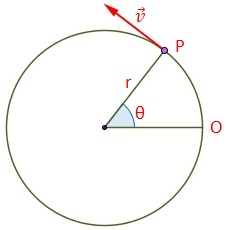
\includegraphics[scale=0.6]{images/movimiento-circular.jpg}
 % cinematica.png: 0x0 px, 300dpi, 0.00x0.00 cm, bb=
 \caption{Ilustración del movimiento circular.}\label{circular}
\end{figure}   

Ya que el cuerpo se mueve a tráves de la trayectoria circular posee dos velocidades: una angular y otra lineal.\\

\subsection{Velocidad angular:}

Esta velocidad mide el ritmo de cambio del ángulo recorrido por el cuerpo en movimiento con respecto al tiempo:

\begin{equation}
\omega = \frac{\Delta \theta}{\Delta t} \quad [rad/s]
\end{equation}

\subsection{Velocidad Lineal:}

También llamada velocidad tangencial mide el ritmo de cambio de la longitud de arco recorrida por el cuerpo con respecto al 
tiempo.

\begin{equation}
v = \frac{\Delta s}{\Delta t} = \frac{R\Delta \theta}{\Delta t} = R\omega \quad [m/s]
\end{equation}

Esta velocidad depende exclusivamente de la velocidad angular de manera directa.\\

También se definen dos magnitudes importantes para este movimiento:\\

\textbf{Período:} es el tiempo $T$ que tarda la partícula en dar una vuelta a la circunferencia completa.\\

\textbf{Frecuencia:} Es el número de vueltas $f$ que recorre la partícula en una unidad de tiempo. Se expresa en ciclos/s o 
hertzios (Hz).\\

Estas dos cantidades se relacionan de manera inversa:

\begin{equation}
f = \frac{1}{T}\quad [Hz]
\end{equation}
, y también con la velocidad angular: 
\begin{equation}
w = 2\pi f = \frac{2\pi}{T}
\end{equation}

Cuando un móvil se mueve con movimiento circular su velocidad lineal siempre esta en constante cambio de dirección, y como se 
sabe que siempre el cambio de velocidad en el tiempo esta medido por una aceleración, y esta aceleración se llama aceleración 
centrípeta.

\subsection{Aceleración centrípeta:}

\begin{figure}[ht]
 \centering
 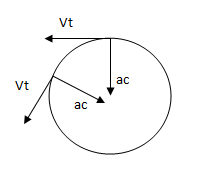
\includegraphics[scale=0.6]{images/aceleracion-centripeta.jpg}
 % cinematica.png: 0x0 px, 300dpi, 0.00x0.00 cm, bb=
 \caption{Ilustración de a aceleración centrípeta.}\label{ac}
\end{figure}

Esta aceleración es la que se origina debido al cambio de dirección constante de la velocidad lineal cuando el cuerpo gira a 
través de la circunferencia, y su dirección es central, siempre apuntando al centro del círculo. Y su expresión de cálculo es:

\begin{equation}
a_c = \frac{v^2}{R} =  \omega^2 R\quad [m/s^2]
\end{equation}

\begin{figure}[ht]
 \centering
 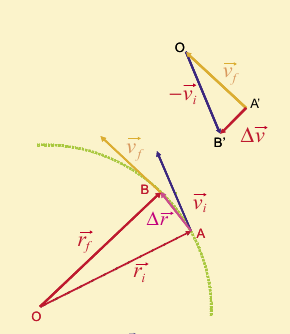
\includegraphics[scale=0.6]{images/acentripeta.png}
 % cinematica.png: 0x0 px, 300dpi, 0.00x0.00 cm, bb=
 \caption{Ilustración del origen vectorial de la aceleración centrípeta.}\label{ac}
\end{figure} 

\section{Movimiento Circular Uniforme (MCU):}

Es aquel movimiento circular en que el móvil se mueve con velocidad tanto angular y lineal constante, es decir la velocidad 
angular y la lineal no cambian su valor en el tiempo. De este modo se puede decir que el móvil en este movimiento recorre 
distancias iguales en tiempo iguales. 

\begin{tcolorbox}
Es decir, en el MCU: $\omega = constante$ y $v = constante.$
\end{tcolorbox}

Esto implica que el cuerpo que tiene MCU sólamente posee una aceleración que es la centrípeta.

\subsection{Problemas de mcu}

\begin{enumerate}
\item Tranformar los siguientes ángulos en radianes:
\begin{itemize}
 \item[a.] $40^\circ$
 \item[b.] $140^\circ$
 \item[c.] $155^\circ$
 \item[d.] $640^\circ$
 \item[e.] $60^\circ$
 \item[f.] $40^\circ$
 \item[g.] $55^\circ$
 \item[h.] $64^\circ$
\end{itemize}

 \item Encontrar la longitud de arco de circunferencia de radio y ángulo:
\begin{itemize}
 \item[a.] 20 cm y $45^\circ$
 \item[b.] 5.0 km y $75^\circ$
 \item[c.] 30 m y $360^\circ$
 \item[d.] 6.5 m y $60^\circ$
  \item[e.] 200 cm y $45^\circ$
 \item[f.] 50.0 km y $75^\circ$
 \item[g.] 77 cm y $360^\circ$
 \item[h.] 50 mm y $60^\circ$
\end{itemize}

\item Una partícula gira por una trayectoria circular de radio 1m da 40 vueltas en 6 segundos. Calcular: a) la velocidad angular 
y b) la aceleración centrípeta.

\item  Una partícula gira por una trayectoria circular de radio 1m da 40 vueltas en 6 segundos. Calcular: a) la velocidad 
angular y b) la aceleración centrípeta.

\item  Un móvil se mueve en una circunferencia de 50 cm de radio con una velocidad angular de 180 rpm, determine la distancia 
recorrida y la frecuencia alcanzada después de 10s.


\item  Del problema anterior encuentre lo siguiente: a) La frecuencia y b) el ángulo girado luego de un minuto.


\item Un punto de la periferia de la rueda de un automóvil con radio 0,30 m se mueve con una velocidad de 36 km/h. ¿Cuál es su 
velocidad angular en rad/s? ¿Cuál es su aceleración centrípeta? 

\item Las aspas de un ventilador giran uniformemente a razón de 90 vueltas por minuto. Determina: a) su velocidad angular, en 
rad/s; b) el número de vueltas que darán las aspas en 5min; c) Su periodo y d) su frecuencia.

\item Un móvil se mueve en una circunferencia de 50 cm de radio con una velocidad angular de 180 rpm/min, determine la distancia 
recorrida y la frecuencia alcanzada después de 10s

 \item Un ciclista recorre 5,4 km en 15 min a velocidad constante. Si el diámetro de las ruedas de su bicicleta es de 80 cm, 
calcula: a) la velocidad angular de las ruedas y b) el número de vueltas que dan las ruedas en ese tiempo.

\item Dos poleas de 6 y 15 cm de radio respectivamente, giran conectadas por una banda. Si la velocidad angular de la polea de 
menor radio es 20 vueltas/segundo. ¿Cúal es la velocidad angular de la polea de radio mayor?.
\begin{figure}[H]
 \centering
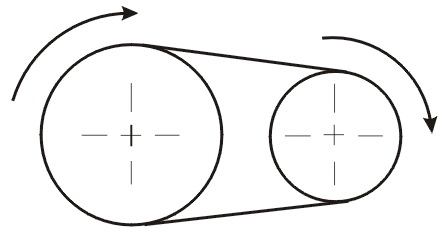
\includegraphics[width=5.0cm,height=3.0cm]{images/poleas.jpg}
\end{figure}

\item Un auto se mueve alrededor de una pista circular cuyo radio es de 50 metros de radio con un velocidad constante de 90 km/h.
 ¿Cuál es la velocidad angular que posee ese auto?
 
\item La rueda de una bicicleta tiene 30 cm de radio y gira uniformemente a razón de 25 vueltas por minuto. Calcula: a) La 
velocidad angular, en rad/s, b) La velocidad lineal de un punto de la periferia de la rueda, c) Ángulo girado por la rueda en 30 
segundos y d) número de vueltas en ese tiempo.

\item Un coche circula a una velocidad de 90 Km/h , si el radio de las ruedas del coche es de 30 cm, calcula: a)su velocidad 
lineal en m/s y b)la velocidad angular de las ruedas en rad /s y r.p.m.

\item  Si la velocidad angular de un disco se duplica, ¿Qué ocurre con la velocidad lineal?
 
\item Un astronauta da la vuelta a la Tierra cada 300 minutos.¿Cuál es la velocidad angular?¿Cuál es su velocidad lineal si 
describe una orbita de 30000 km de radio?

\item ¿Cuál es la velocidad de un angular de un disco que gira con una velocidad angular de 13,4 rad en un minuto? Si el radio 
del disco es 20 cm, ¿cuál es la velocidad lineal en el borde del mismo?.

\item ¿Cuánto tiempo necesitará el disco anterior para girar 3 vueltas enteras?¿Cuál es la aceleración centrípeta en el borde del 
disco?

\item ¿Cuál es la velocidad angular de un disco que gira con una velocidad angular de $3\pi$ rad en medio minuto? Si el radio del 
disco es 40 cm, ¿cuál es la aceleración centrípeta en el borde del mismo?.

\item ¿Cuál es la velocidad angular de las manecillas del reloj?¿El periodo del movimiento?

\item Un móvil recorre una circunferencia de 2 m de radio dando 20 vueltas en 10 segundos. Determinar:

\begin{itemize}
 \item [a.] La frecuencia.
 \item [b.] El periodo.
 \item [c.] La velocidad angular.
 \item [d.] La velocidad lineal.
\end{itemize}

\item Calcule la aceleración centrípeta de la   Luna.

\item Calcule la aceleración centrípeta y angular de la Tierra alrededor del Sol.

\item  Un punto de la periferia de la rueda de un automóvil con radio 0,30 m se mueve con una velocidad de 36 km/h. ¿Cuál es su 
velocidad angular en rad/s? ¿Cuál es su aceleración centrípeta?

\item Desde un mismo punto de la circunferencia parten dos móviles en sentido opuesto. El primero recorre la circunferencia en 
1h10 min y el segundo recorre un ángulo de $30^\circ$ en 3 segundos. Determine cuándo se encuentran los móviles.

\end{enumerate}


\section{Movimiento Circular Uniformemente Variado:}

Es el movimiento que realiza un cuerpo con trayectoria circular y con una aceleración tangencial, que hace que la velocidad 
lineal y angular no sean constantes en el tiempo. El cuerpo con MCUV tiene una aceleración angular y aceleración tangencial 
constantes, y estás miden la variación de la velocidad angular y lineal respecto al tiempo.\\

\subsection{Aceleración angular:}

Es una cantidad vectorial que mide el ritmo de cambio de la velocidad angular con el tiempo, la cual se mantiene constante en el 
MCUV. Esta aceleración se calcula así:

\begin{equation}
\alpha = \frac{\Delta \omega}{\Delta t} =  \frac{\omega_f - \omega_0}{\Delta t}\quad [rad/s^2]
\end{equation}
  

donde $\Delta \omega = \omega_f-\omega_0$ representa la variación de la velocidad angular desde una inicial $\omega_0$ hasta una 
final $\omega_f$. Si esta aceleración $\alpha$ es positiva el movimiento es acelerado, mientras que si $\alpha$ es negativa el 
movimiento es de frenado.

\subsection{Aceleración tangencial:}

O también llamada lineal, esta mide la variación de la velocidad tangencial con respecto al tiempo, la cual se mantiene constante 
en el MCUV. Esta aceleración se calcula así:

\begin{equation}
a_T =\frac{\Delta v}{\Delta t} =\frac{v_f-v_0}{\Delta t}\quad [m/s^2]
\end{equation} 

donde $\Delta v = v_f-v_0$ representa la variación de la velocidad tangencial desde una inicial $v_0$ hasta una final $v_f$. Si 
esta aceleración $a_T$ es positiva el movimiento es acelerado, mientras que si $\alpha$ es negativa el movimiento es de frenado. 
Así, mismo como la velocidad tangencial esta aceleración es tangente a la trayectoria, y mide de que tan rápido o tan lento el 
cuerpo está cambiando su velocidad.

\begin{tcolorbox}
En el MCUV: $a_T = constante$ y $\alpha = constante$
\end{tcolorbox}

Las dos aceleraciones anteriores descritas se relacionan mediante la siguiente ecuación:

\begin{equation}
a_T = \alpha R
\end{equation} 

, y la aceleración resultante de un cuerpo con MCUV es:

\begin{equation}
\vec{a} = \vec{a_T}+\vec{a_c}
\end{equation}

cuyo módulo es entonces:

\begin{equation}
a_R =\sqrt{a_c^2+a_T^2} 
\end{equation}

\begin{figure}[ht]
 \centering
 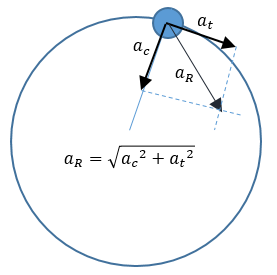
\includegraphics[scale=0.5]{images/aceleracion-resultante.png}
 % cinematica.png: 0x0 px, 300dpi, 0.00x0.00 cm, bb=
 \caption{Ilustración de la aceleración resultante en un MCUV.}\label{ac}
\end{figure} 
 
Este movimiento queda descrito completamente con las siguientes ecuaciones:\\

\textbf{Parte angular:}

\begin{equation}
\omega_f = \omega_0 + \alpha t
\end{equation}

\begin{equation}
\omega_f^2 = \omega_0^2 + 2\alpha\theta
\end{equation}

\begin{equation}
\theta = (\frac{\omega_f + \omega_0}{2})t
\end{equation}

\begin{equation}
\theta = \omega_0t+\frac{1}{2}\alpha t^2
\end{equation}

\textbf{Parte lineal:}

\begin{equation}
v_f = v_0 + a_Tt
\end{equation}

\begin{equation}
v_f^2 = v_0^2 +2a_Ts
\end{equation}

\begin{equation}
s = (\frac{v_f + v_0}{2})t
\end{equation}

\begin{equation}
s = v_0t+\frac{1}{2}a_Tt^2
\end{equation}


\section{Problemas de mcuv}

\begin{enumerate}

\item Una partícula inicia su M.C.U.V. con una velocidad tangencial de 6 m/s. Si su aceleración tangencial es $4 m/s^2$, y su 
radio de giro es 9 m. Determinar su velocidad tangencial y angular luego de 12 segundos.

\item Calcular la aceleración angular que tiene un disco, sabiendo que éste es capaz de triplicar la velocidad que tiene luego de 
dar 600 vueltas en 20 s.

\item La velocidad de una rueda, que gira con movimiento uniformemente retardado, disminuyó al ser frenada durante 1 minuto, 
desde 
300 R.P.M. hasta 180 R.P.M. Hallar la aceleración angular de la rueda.

\item Un ventilador alcanza su velocidad máxima de trabajo de 900 R.P.M. en 40 s. Si al ``encenderlo'' inicia su movimiento con 
aceleración constante, calcular cuántas revoluciones completa en el primer minuto de su movimiento.

\item La velocidad angular de un motor cambia uniformemente
 200 rpm a 120 rpm en 4 segundos. Determinar: a) la aceleración 
angular y b) el
 desplazamiento angular.

\item  La velocidad de
 un automóvil aumenta en 5 segundos de 15 km/h a 55 km/h. Si el radio de las ruedas es de 70
 cm, ¿cuál es 
la aceleración angular de las mismas? 

\item Un móvil tiene una velocidad tangencial de 120m/s; luego de 5 segundos esta velocidad se convierte en 154 m/s. Si el radio 
de la circunferencia es de 4m, hallar la aceleración angular. 

\item Una rueda de 50cm de diámetro tarda 10 segundos en adquirir una velocidad constante de 360rpm. Calcula la aceleración 
angular y la aceleración centrípeta que posee un punto en la periferia de la rueda a los 5 segundos la rueda del problema.

\item Un volante de 50cm de radio gira a 180 rpm. Si es frenado y se detiene en 20 segundos, calcula: a) La velocidad angular 
inicial en radianes por segundo, y b) La aceleración tangencial de frenado.

\item Calcular la  velocidad  angular  final  y  el desplazamiento  angular de  una  rueda  que  tiene una velocidad angular 
inicial de $8 rad/s$ y experimenta una aceleración de $3 rad/s^2$ en 12 s.

\item Una  rueda  gira  con  una  velocidad  angular inicial  de  12  rad/s  experimentando  una  aceleración de $5 rad/s^2$ en 
6s. Calcular: a) el desplazamiento angular total, b) la velocidad angular final.

\item La velocidad angular de un motor cambia uniformemente 200 rpm a 120 rpm en 4 segundos. Determinar la aceleración lineal de 
un punto que esta a 50 cm del eje de rotación del motor.

\item Un punto de la periferia de la rueda de un automóvil con radio 0,30 m  se mueve con una velocidad de 72 km/h, de pronto el 
automóvil se frena uniformemente a razón de $4 m/s^2$.  Calcular  el ángulo girado  después de 10 segundos.

\item  Un motor que tiene 
una frecuencia de 20 Hz, se apaga y se detiene en 5 segundos. ¿Cuál es su velocidad lineal al 

tiempo de 2 segundos de un punto que se ubica a 50 cm del eje de rotación del motor?

\end{enumerate}
